\section{Langkah-Langkah Percobaan}
Dilakukan dua percobaan dalam praktikum ini. Percobaan pertama adalah melakukan 
crimping pada kabel UTP, sedangkan percobaan kedua adalah melakukan routing 
IPv4 secara statis dan dinamis.

\begin{enumerate}
    \item \textbf{Percobaan 1: Crimping}
    \begin{enumerate}
        \item Siapkan alat dan bahan yang dibutuhkan, seperti 
        kabel LAN, konektor, crimping tool, dan tester.
        \item Potong kabel LAN dengan panjang yang diinginkan.
        \item Kupas ujung kabel LAN sekitar 2-3 cm dengan 
        crimping tool untuk mengeluarkan kawat-kawat di dalamnya.
        \begin{center}
		    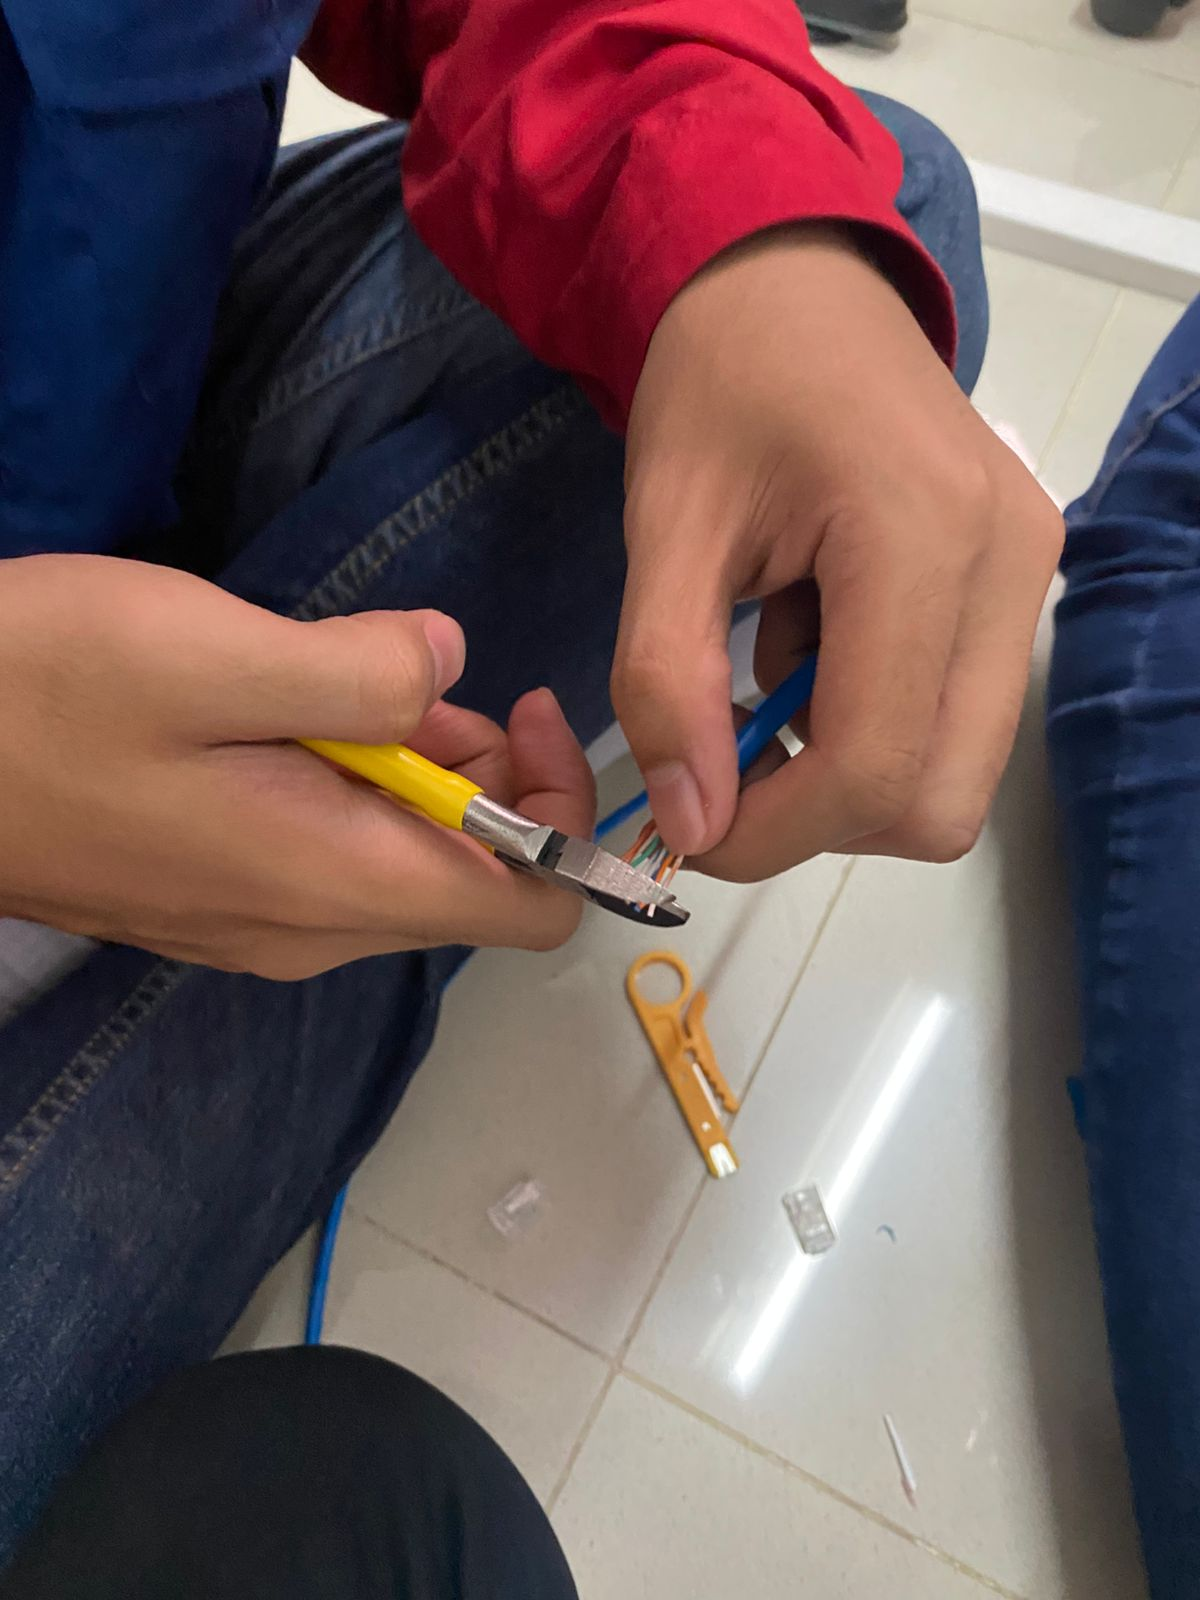
\includegraphics[scale=0.1]{P1/img/1-5.jpg}
        \end{center}
        \item Urutkan kawat-kawat sesuai dengan standar T568B.
        \begin{center}
		    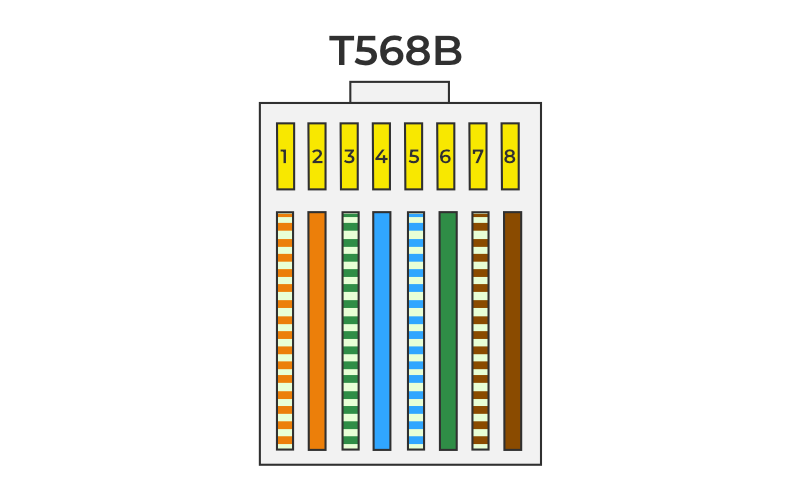
\includegraphics[scale=0.4]{P1/img/crimping.png}
        \end{center}
        \item Masukkan kawat-kawat ke dalam konektor sesuai 
        urutan yang telah ditentukan.
        \item Gunakan crimping tool untuk menekan konektor ke 
        kabel LAN.
        \item Uji koneksi menggunakan tester untuk memastikan 
        semua kawat terhubung dengan baik.
        \begin{center}
		    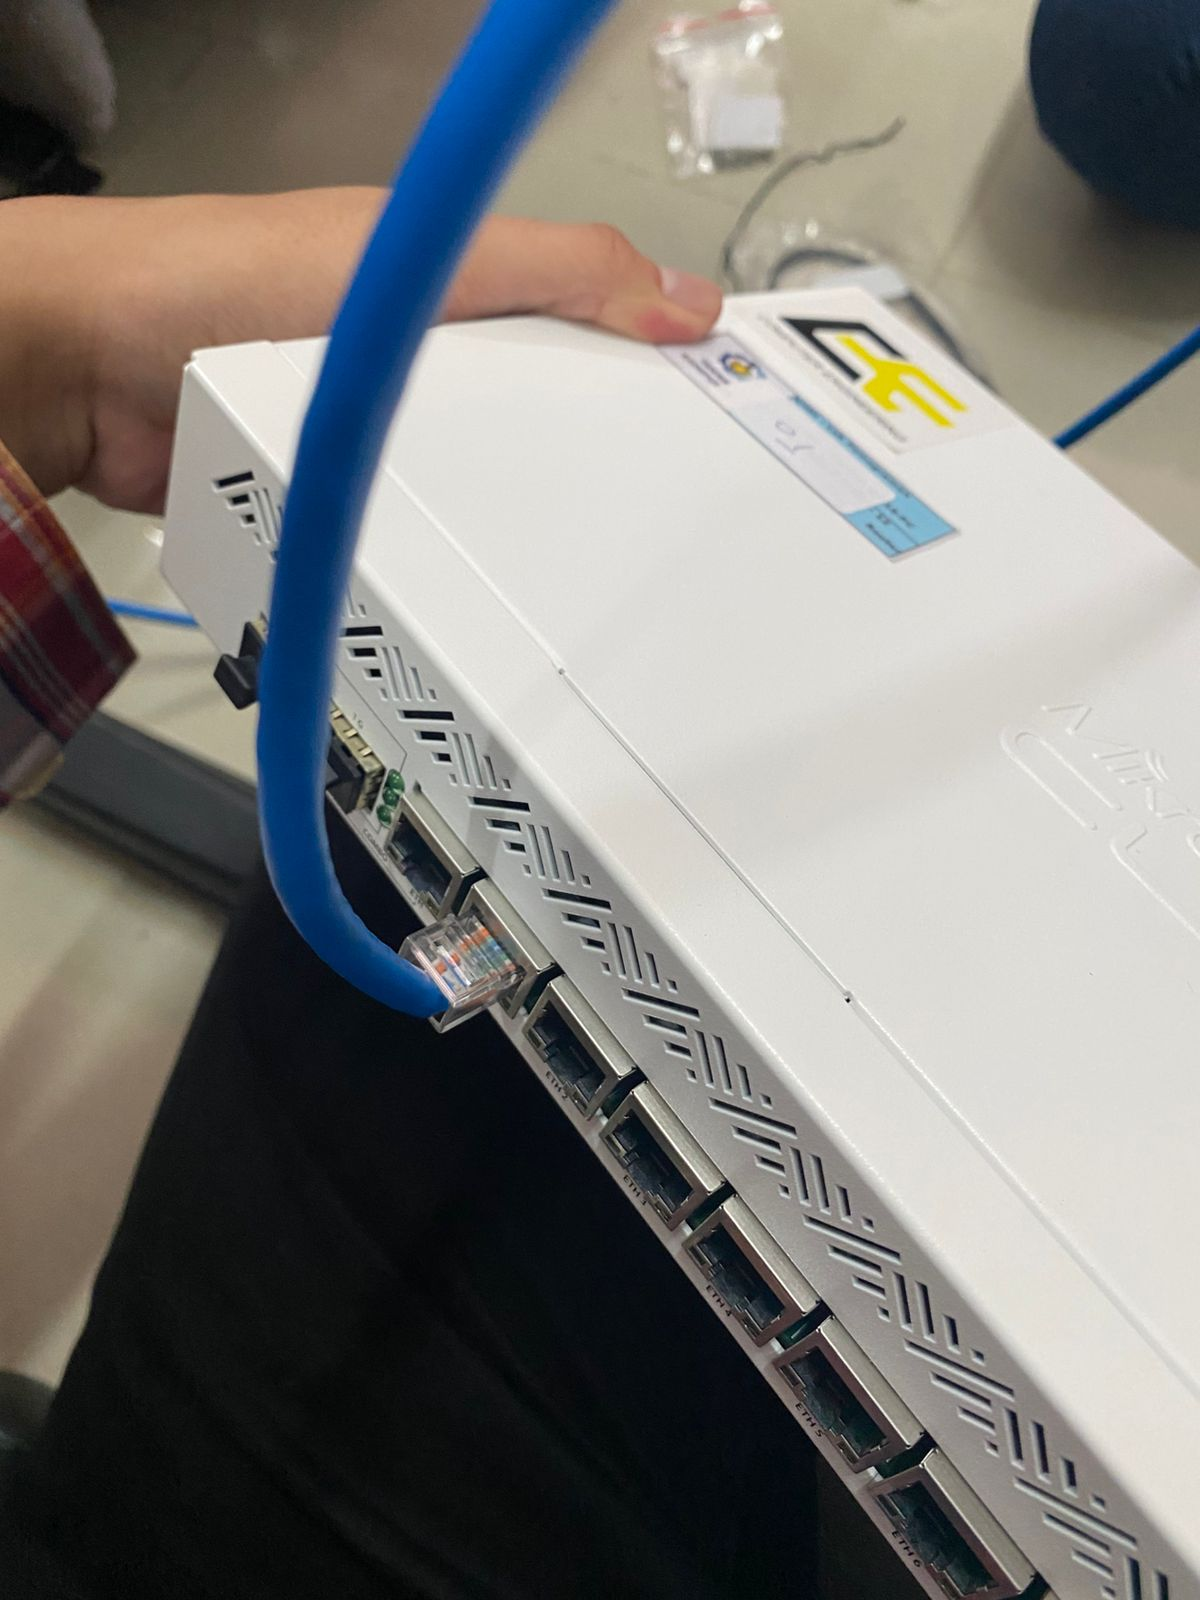
\includegraphics[scale=0.1]{P1/img/1-6.jpg}
        \end{center}
    \end{enumerate}
    \item \textbf{Percobaan 2: Routing IPv4 -- Statis}
    \begin{enumerate}
        \item Siapkan dua perangkat router, dua laptop dengan winbox 
        MikroTik, dan kedua kabel LAN yang telah dibuat.
        \item Hubungkan kedua laptop ke dua router berbeda dengan kabel LAN 
        yang telah dibuat.
        \begin{center}
		    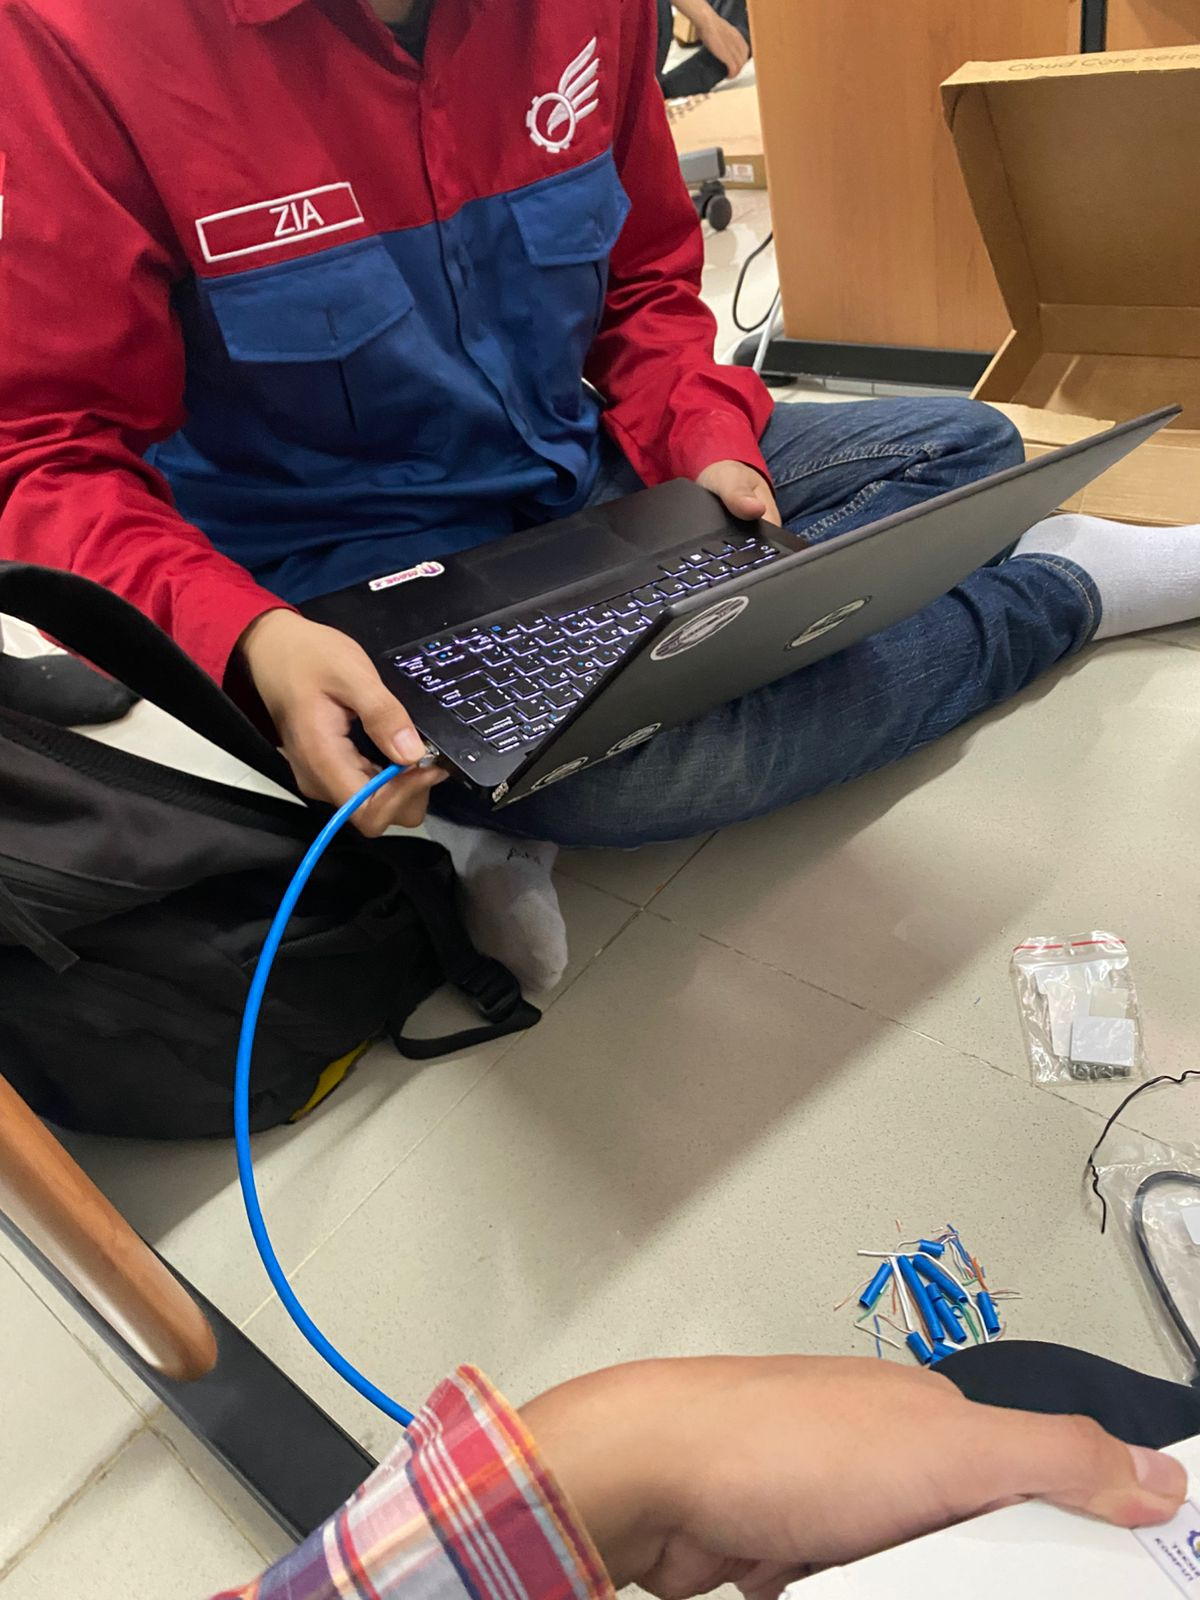
\includegraphics[scale=0.1]{P1/img/1-7.jpg}
        \end{center}
        \item Jalankan winbox pada laptop 
        \begin{center}
		    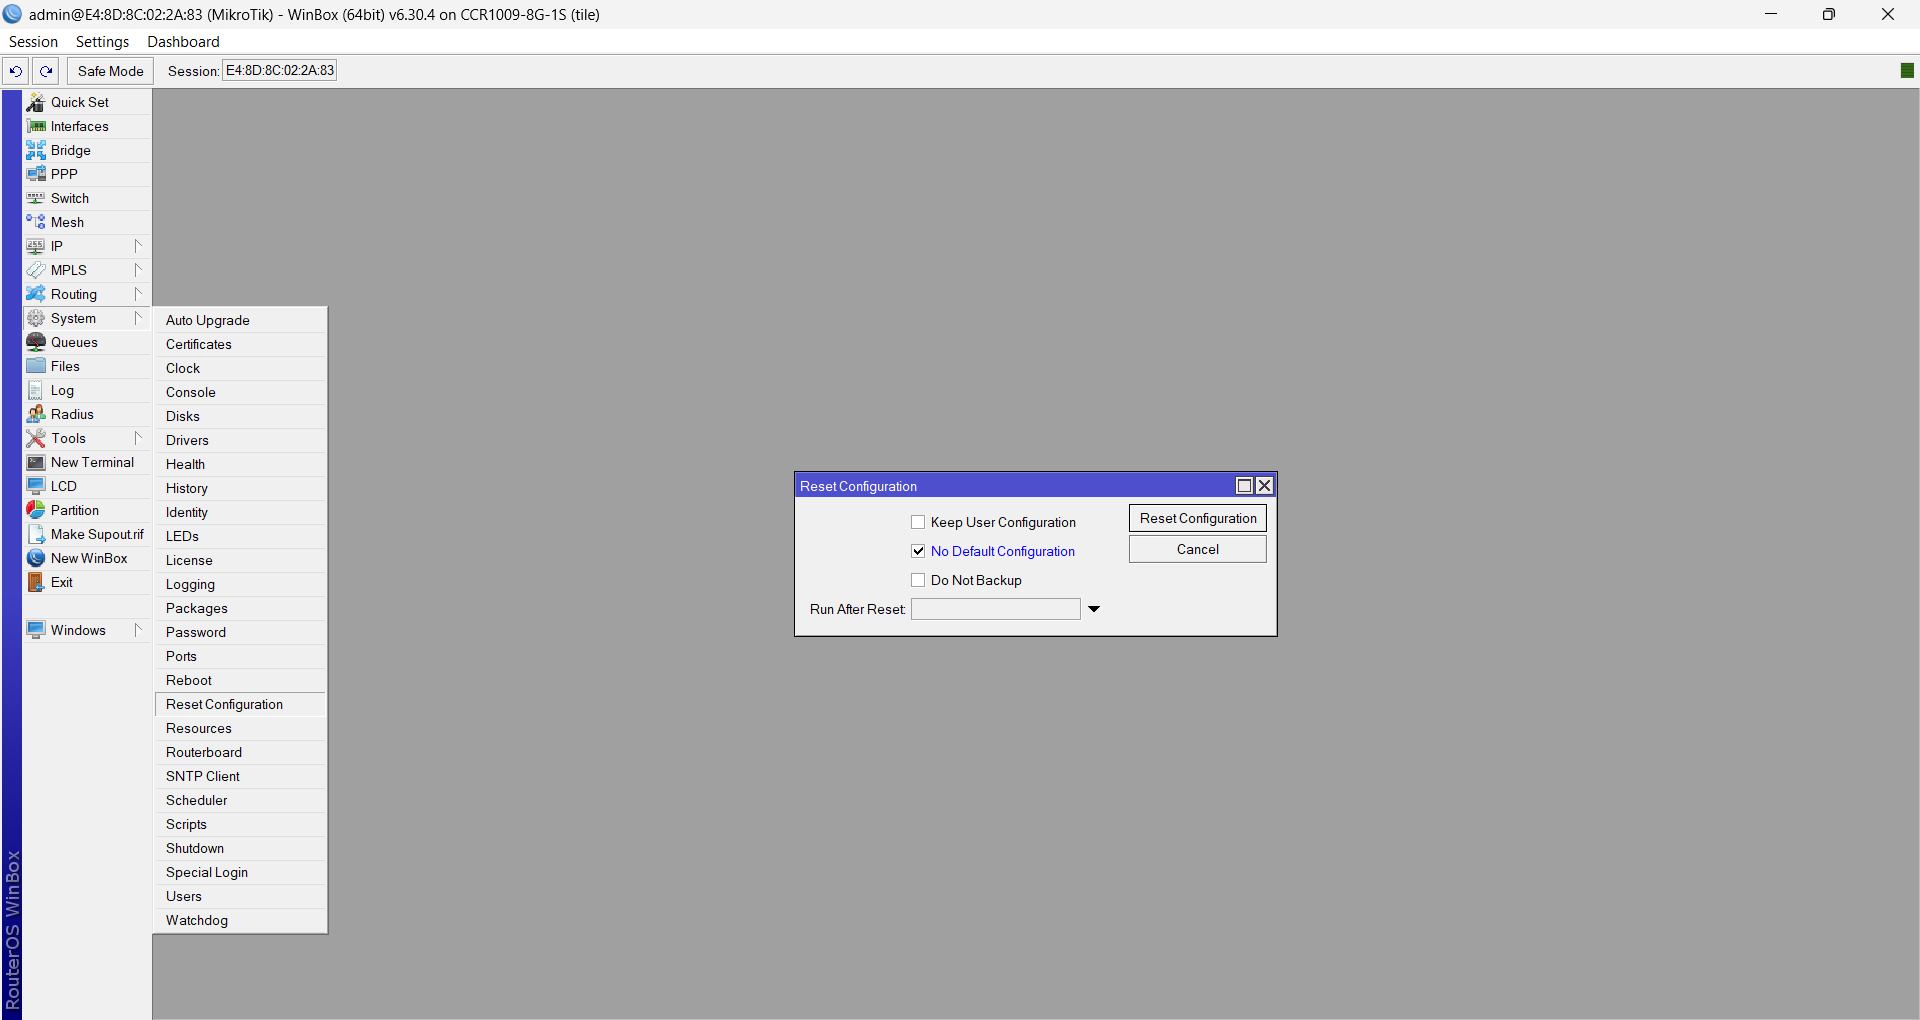
\includegraphics[scale=0.17]{P1/img/1-11.png}
        \end{center}
        \item Atur IP address
        pada masing-masing laptop dan router serta tentukan port ethernet
        berapa saja yang digunakan pada masing-masing router.
        Konfigurasi alamat IP pada masing-masing 
        interface router sesuai dengan subnet yang telah 
        ditentukan. Alamat-alamat IP tersebut adalah sebagai
        berikut:
        \item Atur alamat IP pada setiap interface router berdasarkan konfigurasi subnet yang dibutuhkan. Gunakan subnet yang sama seperti pada percobaan perutean statis:
        \begin{itemize}
            \item Router 1:
            \begin{itemize}
                \item Alamat IP: 192.168.10.1
                \item Netmask: 255.255.255.240
            \end{itemize}
            \item Router 2:
            \begin{itemize}
                \item Alamat IP: 192.168.20.1
                \item Netmask: 255.255.255.240
            \end{itemize}
            \item Router harus terhubung bersama pada antarmuka bersama (mis., ether2 pada kedua router) menggunakan subnet perantara, seperti:
            \begin{itemize}
                \item Router 1 ether2: 10.0.0.1/30
                \item Router 2 ether2: 10.0.0.2/30
            \end{itemize}
        \end{itemize}
        \begin{center}
		    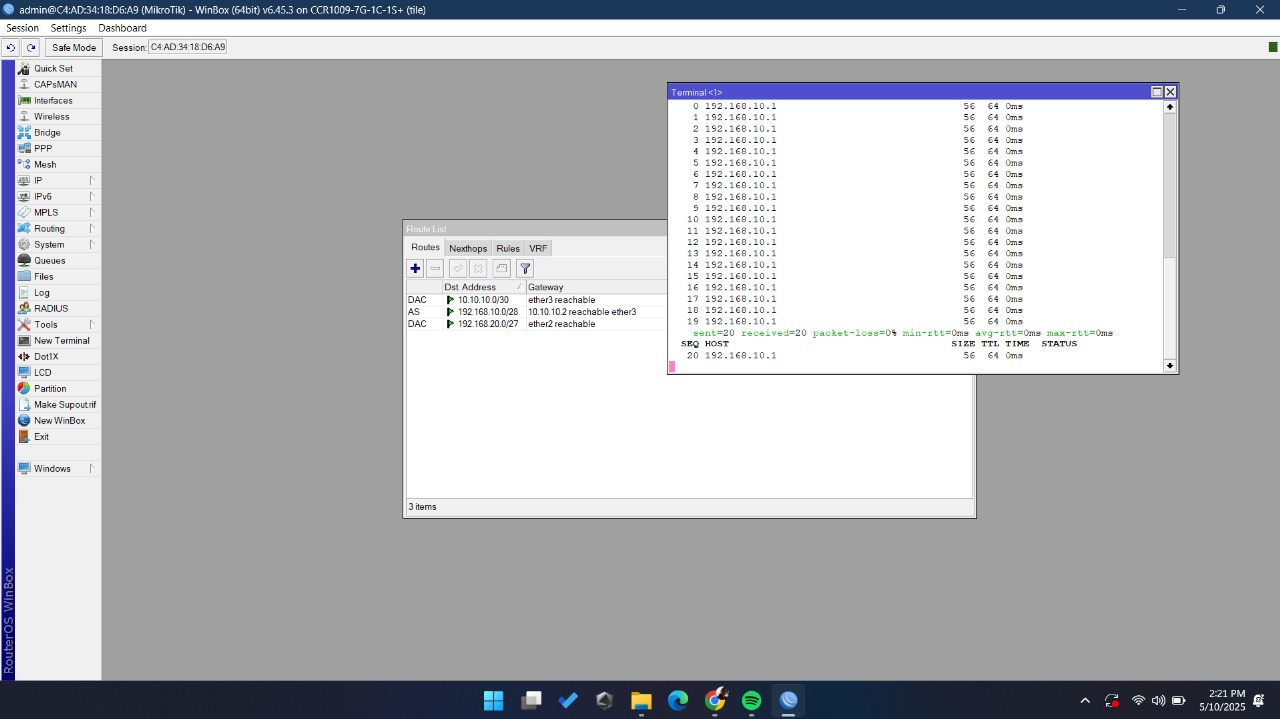
\includegraphics[scale=0.4]{P1/img/1-2.jpg}
        \end{center}
        \item Setelah IP router terkonfigurasi, bisa dilanjut untuk 
        mengatur IP address pada masing-masing laptop sesuai dengan
        subnet yang telah ditentukan. Alamat-alamat IP tersebut adalah
        sebagai berikut:
        \begin{itemize}
            \item Router 1 (tersambung ke laptop 1):
            \begin{itemize}
                \item IP Address: 192.168.10.2
                \item Netmask: 255.255.255.240
                \item Gateway: 192.168.10.1
                \item DNS: 8.8.8.8 (Google DNS)
            \end{itemize}
            \item Router 2 (tersambung ke laptop 2):
            \begin{itemize}
                \item IP Address: 192.168.20.2
                \item Netmask: 255.255.255.240
                \item Gateway: 192.168.20.1
                \item DNS: 8.8.8.8 (Google DNS)
            \end{itemize}
        \end{itemize}
        \begin{center}
		    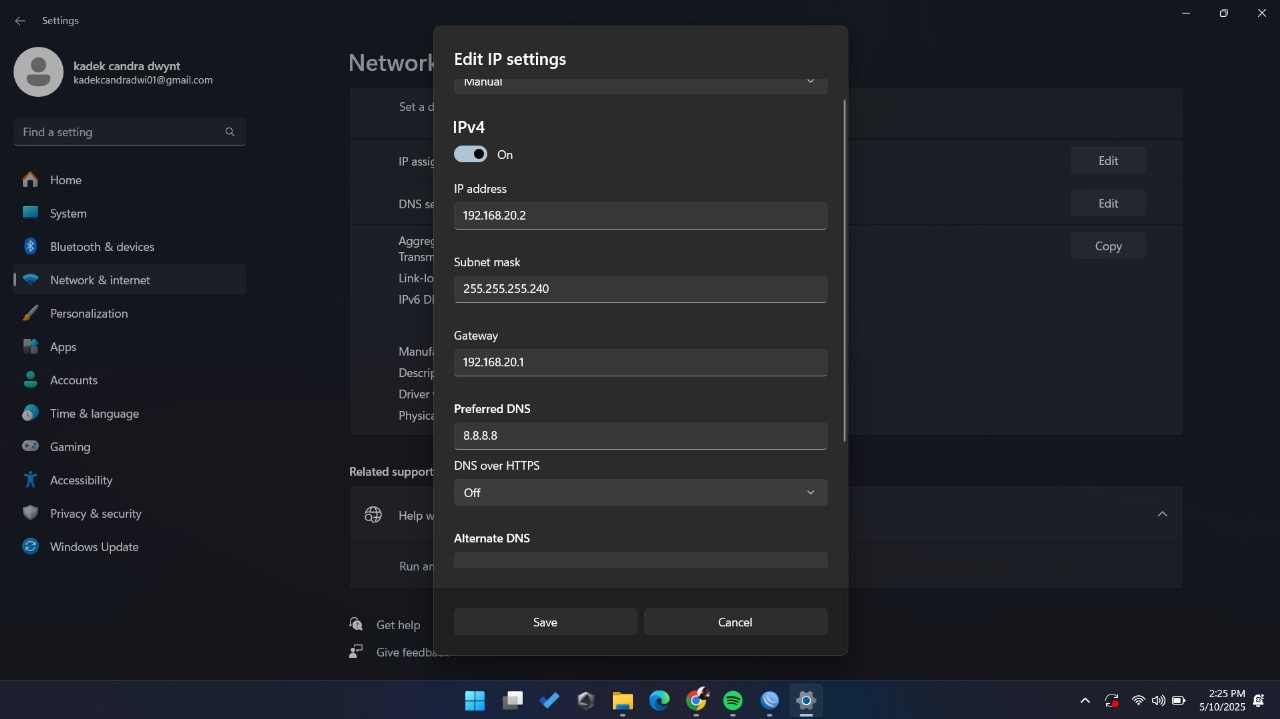
\includegraphics[scale=0.4]{P1/img/1-3.jpg}
        \end{center}
        \item Uji koneksi antar perangkat menggunakan perintah 
        ping di cmd untuk memastikan routing berfungsi dengan 
        baik.
        \begin{center}
		    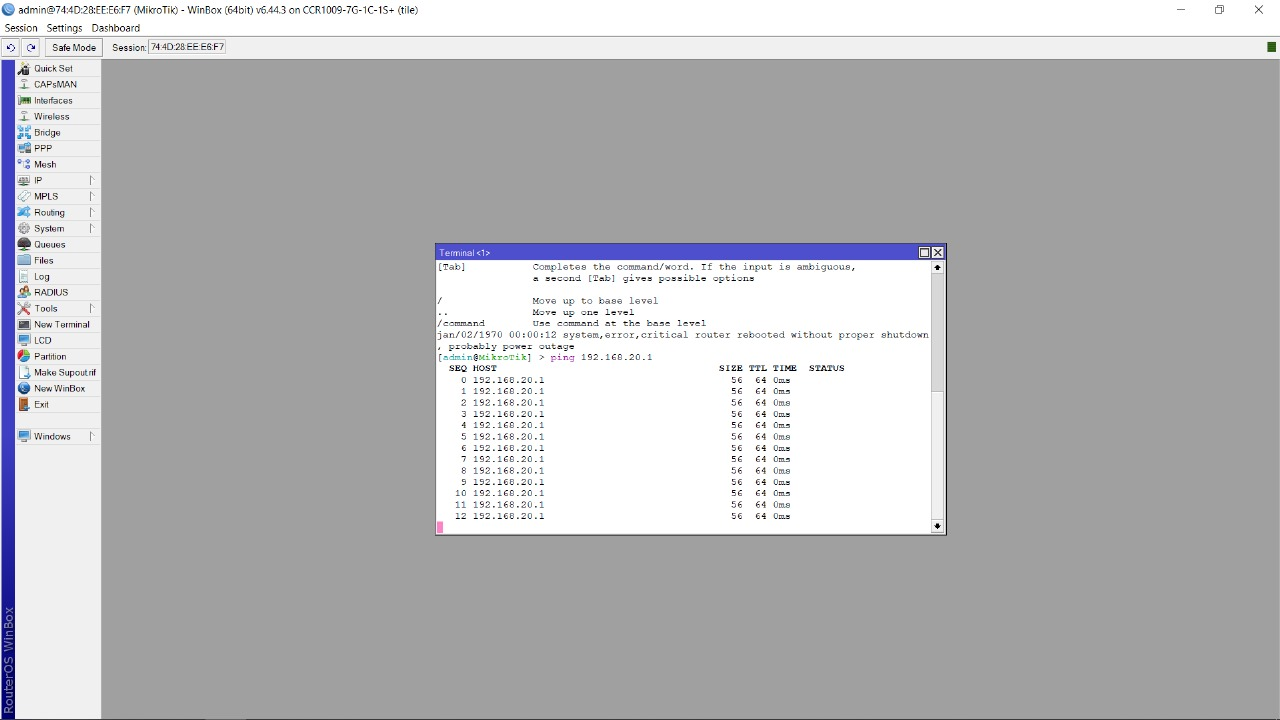
\includegraphics[scale=0.4]{P1/img/1-10.jpg}
        \end{center}
    \end{enumerate}
    \item \textbf{Eksperimen 3: Perutean IPv4 - Dinamis}
    \begin{enumerate}
        \item Siapkan dua perangkat router, dua laptop dengan Winbox, dan kedua kabel LAN yang telah dibuat.
        \item Hubungkan kedua laptop ke dua router yang berbeda dengan menggunakan kabel LAN yang telah dibuat.
        \begin{center}
		    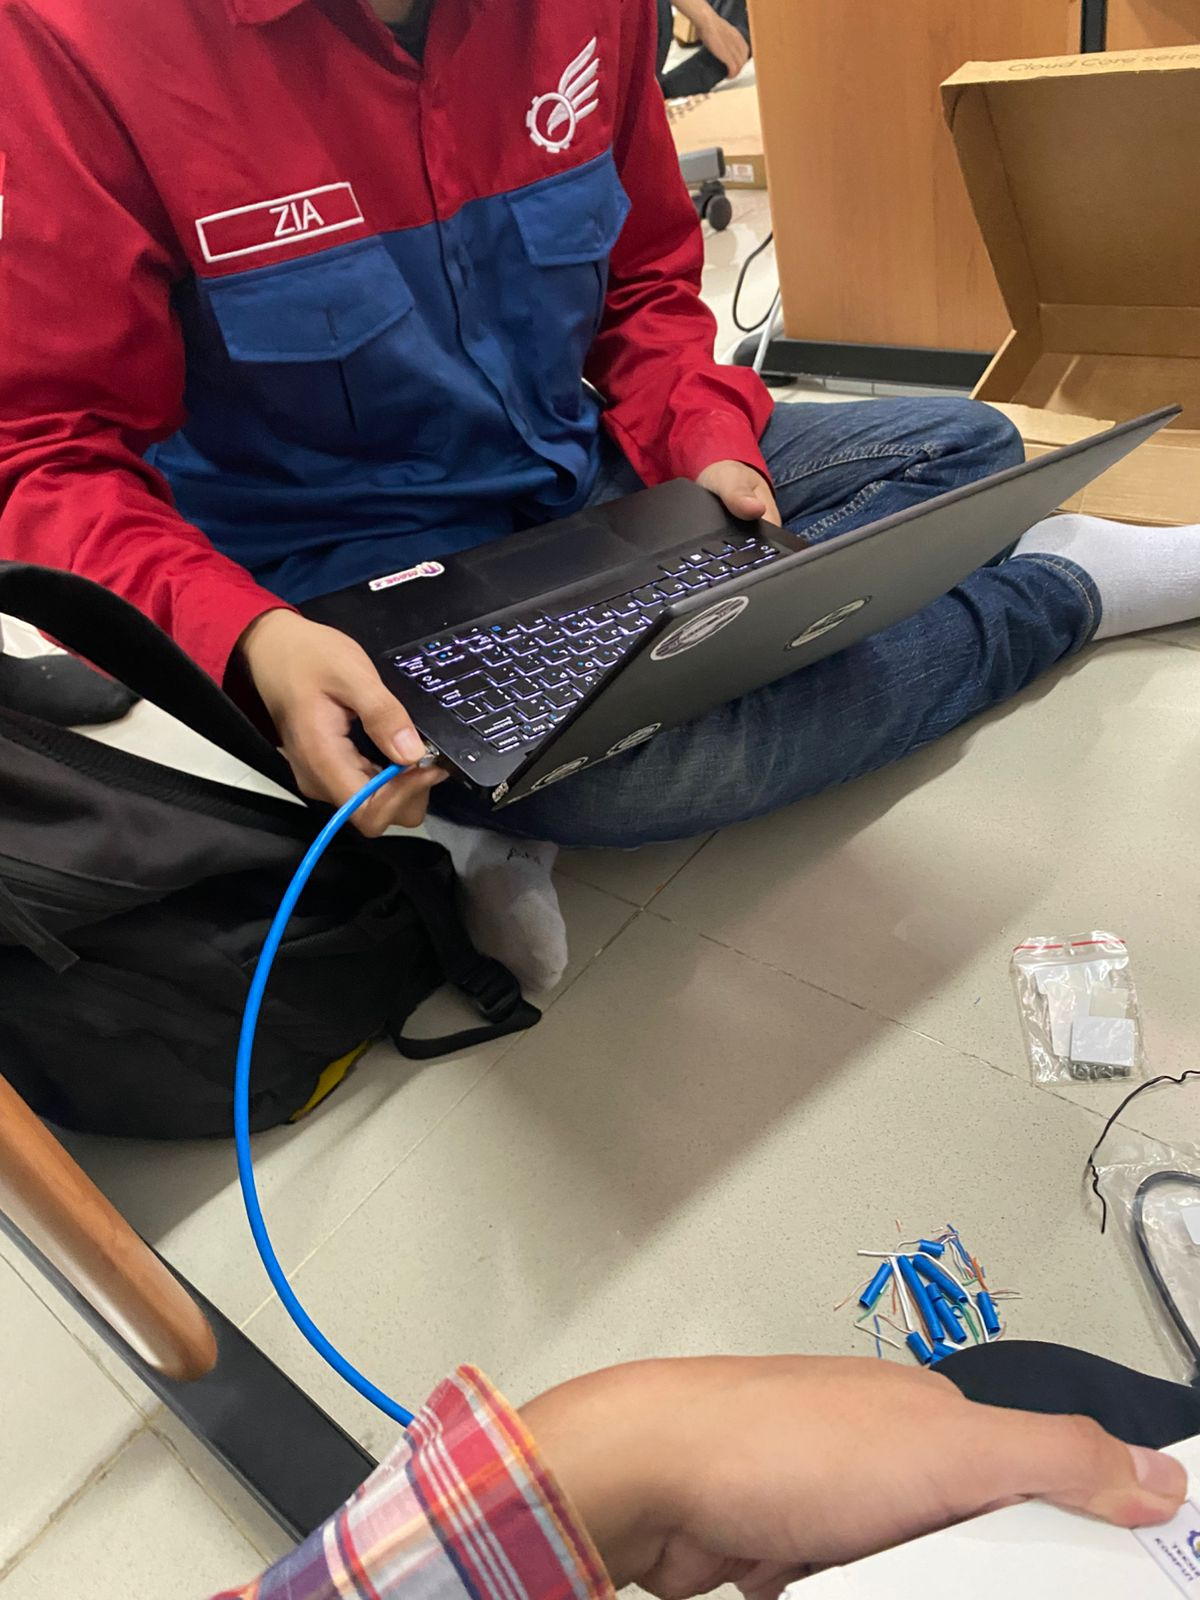
\includegraphics[scale=0.1]{P1/img/1-7.jpg}
        \end{center}
        \item Jalankan Winbox pada masing-masing laptop dan login ke router yang terhubung.
        \begin{center}
		    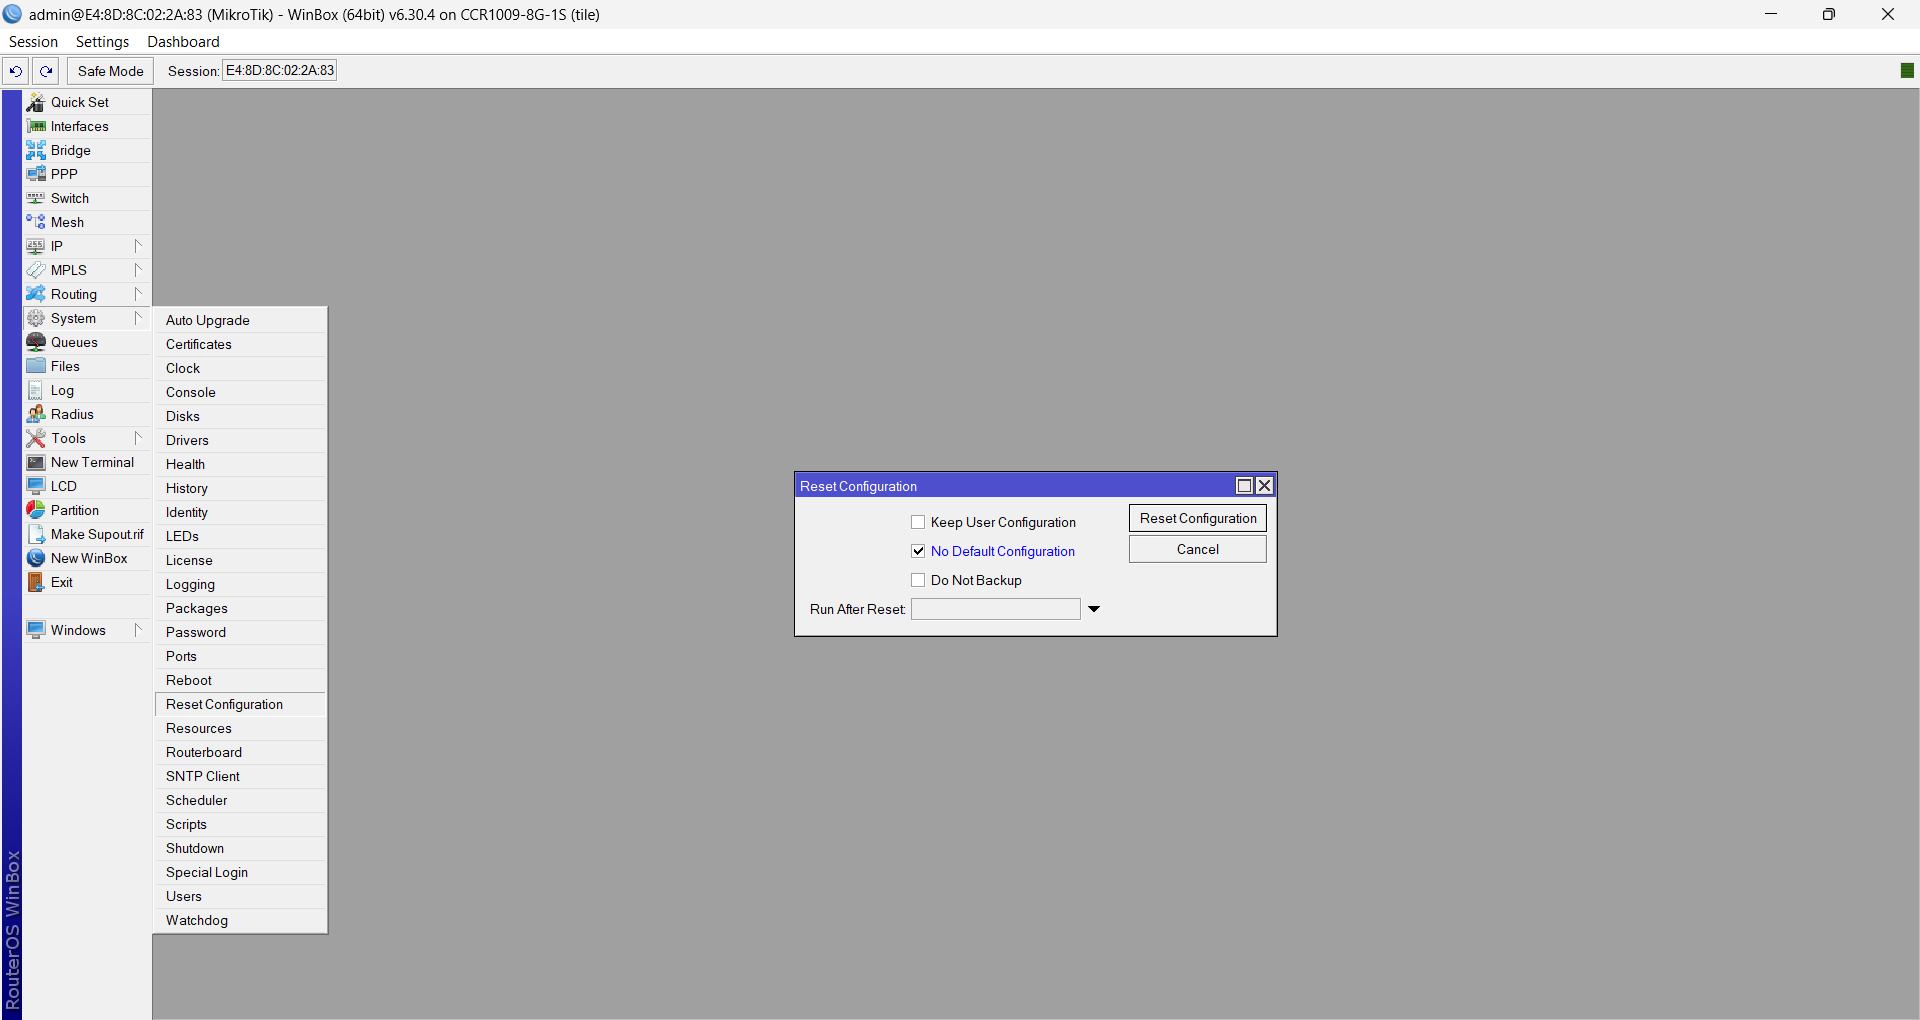
\includegraphics[scale=0.17]{P1/img/1-11.png}
        \end{center}
        \item Aktifkan protokol perutean dinamis RIP pada kedua router:
        \begin{itemize}
            \item Di Winbox, buka \texttt{Routing > RIP}.
            \begin{center}
                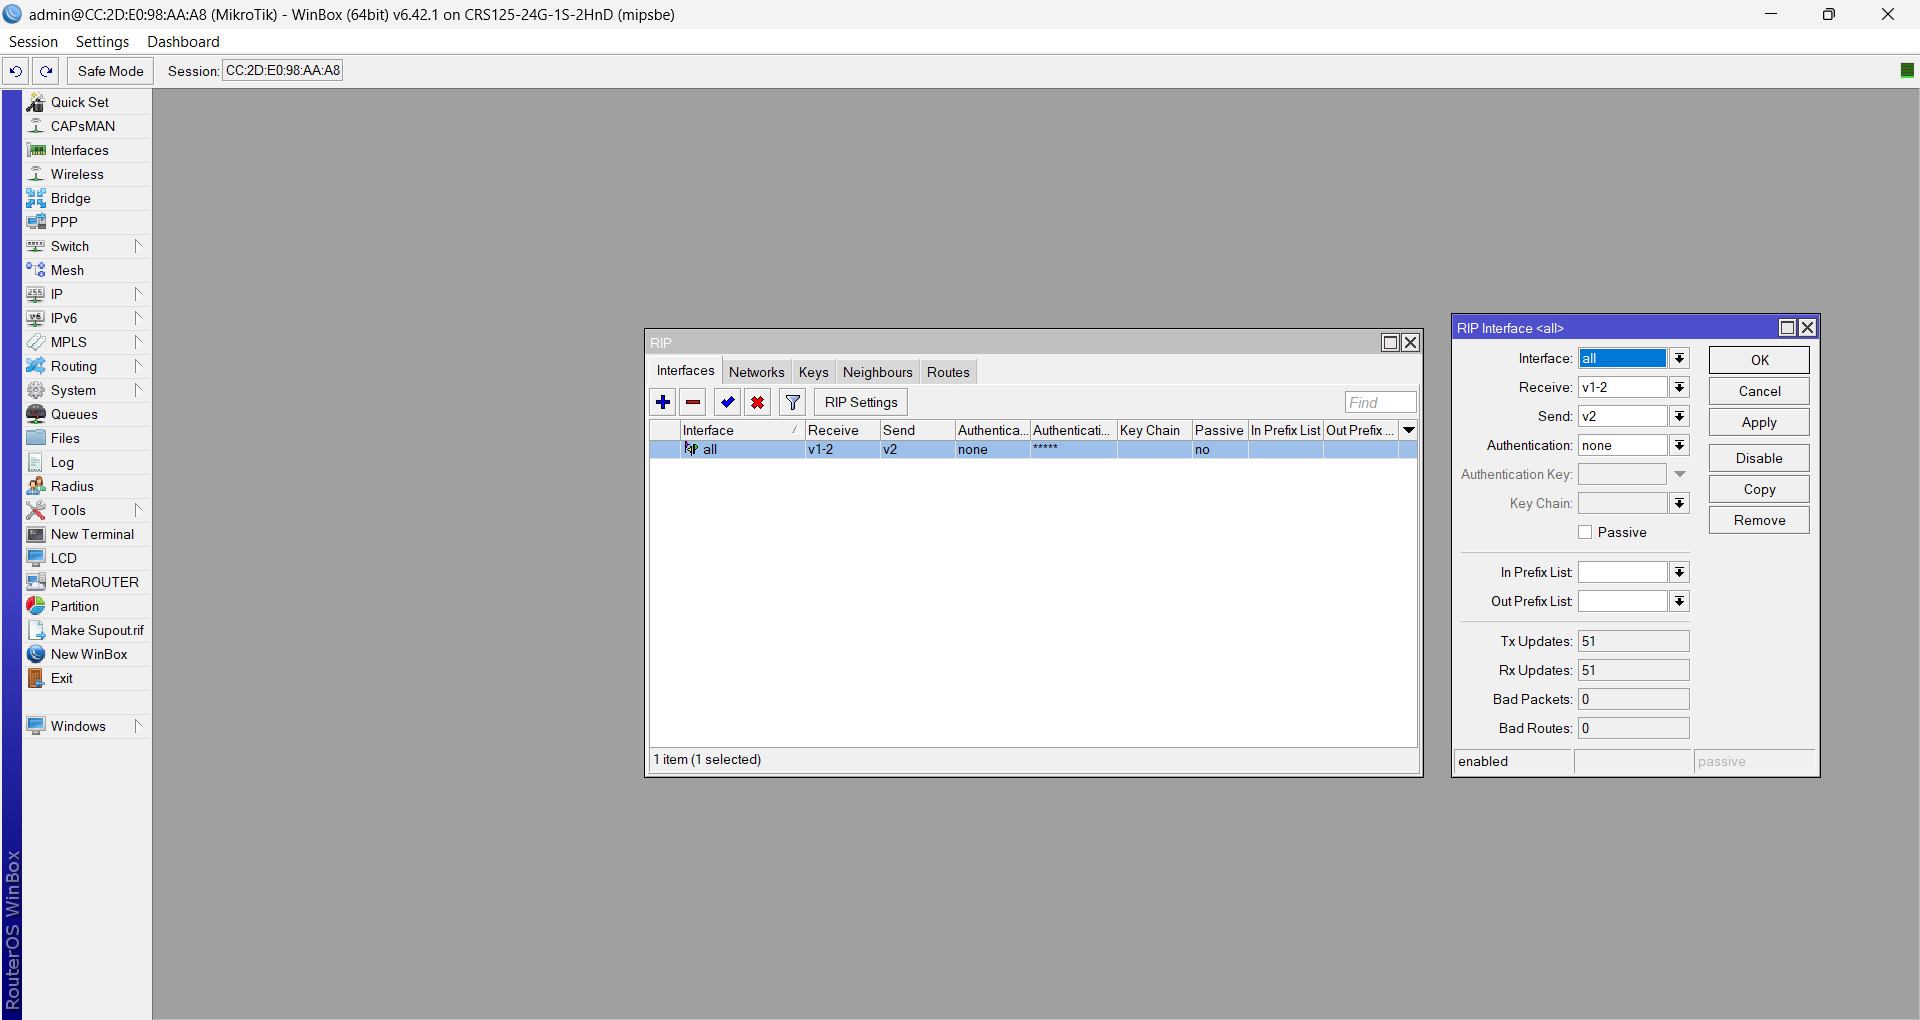
\includegraphics[scale=0.17]{P1/img/1-12.png}
            \end{center}
            \item Tambahkan contoh baru dan tentukan antarmuka yang terhubung.
            \item Pastikan kedua router mengiklankan subnet yang tersambung secara langsung (misal, 192.168.10.0/28, 192.168.20.0/28, dan 10.0.0.0/30).
            \item Terapkan dan verifikasi pembaruan tabel perutean.
        \end{itemize}
        \item Atur alamat IP pada setiap interface router berdasarkan konfigurasi subnet yang dibutuhkan. Gunakan subnet yang sama seperti pada percobaan perutean statis:
        \begin{itemize}
            \item Router 1:
            \begin{itemize}
                \item Alamat IP: 192.168.10.1
                \item Netmask: 255.255.255.240
            \end{itemize}
            \item Router 2:
            \begin{itemize}
                \item Alamat IP: 192.168.20.1
                \item Netmask: 255.255.255.240
            \end{itemize}
            \item Router harus terhubung bersama pada antarmuka bersama (mis., ether2 pada kedua router) menggunakan subnet perantara, seperti:
            \begin{itemize}
                \item Router 1 ether2: 10.0.0.1/30
                \item Router 2 ether2: 10.0.0.2/30
            \end{itemize}
        \end{itemize}
        \item Tetapkan alamat IP pada kedua laptop menjadi DHCP
        \item Gunakan perintah ping di setiap laptop untuk memverifikasi konektivitas ujung ke ujung.
        \begin{itemize}
            \item Dari Laptop 1, lakukan ping ke alamat IP Laptop 2 (192.168.20.2).
            \item Dari Laptop 2, lakukan ping ke alamat IP Laptop 1 (192.168.10.2).
        \end{itemize}
        \begin{center}
		    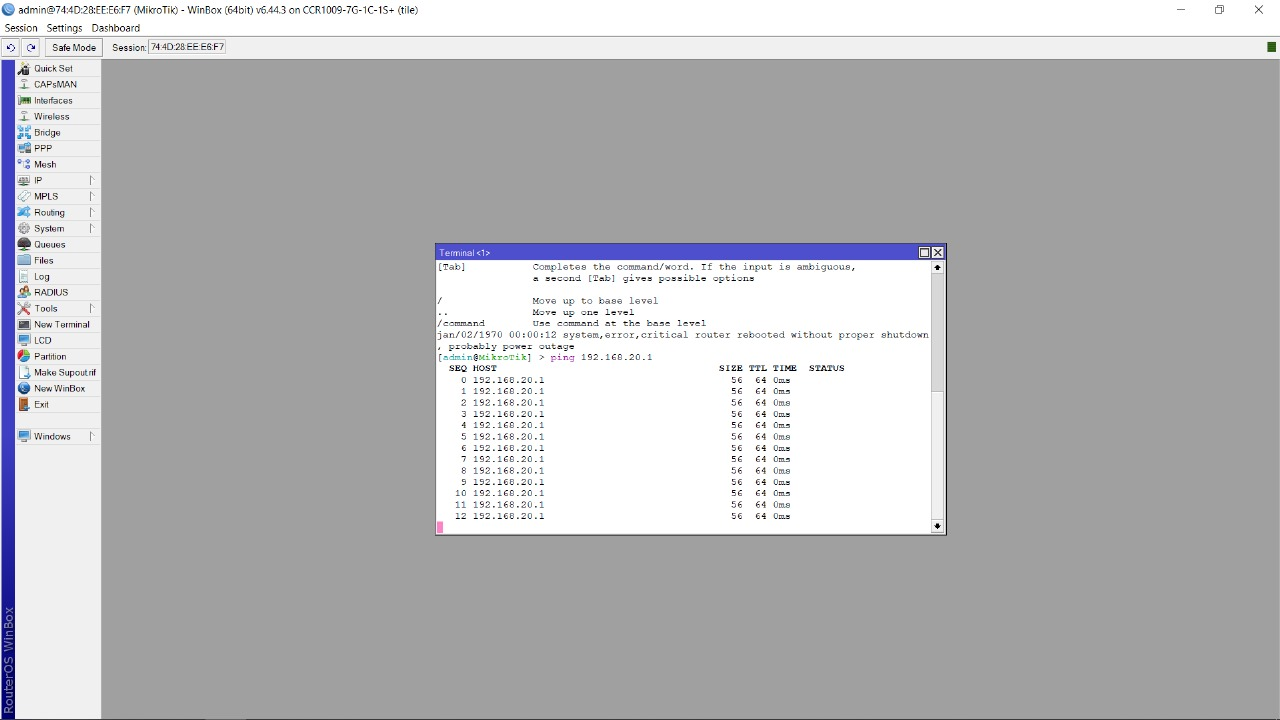
\includegraphics[scale=0.4]{P1/img/1-10.jpg}
        \end{center}
        \item Jika ping berhasil, perutean dinamis bekerja dengan benar.
    \end{enumerate}

\end{enumerate}

\section{Analisis Hasil Percobaan}
\begin{enumerate}
    \item \textbf{Percobaan 1: Crimping}
    
    Tujuan dari percobaan ini adalah untuk membuat kabel LAN 
    yang berfungsi dengan baik yang memungkinkan perangkat 
    terhubung dengan benar. Proses ini memakan waktu lebih lama dari yang 
    diperkirakan karena kesalahan awal saat mengupas jaket luar kabel UTP. 
    Potongannya terlalu dalam sehingga merusak beberapa kabel internal, 
    yang berarti prosesnya harus diulang kembali. Setelah kabel dipangkas 
    dan disusun dengan benar sesuai dengan standar, kabel diuji dengan 
    menggunakan penguji LAN. Alat ini memeriksa apakah konektor RJ45 
    terhubung dengan benar-jika kedelapan lampu indikator menyala secara 
    berurutan, maka kabel dipastikan berfungsi dengan baik. Kesalahan ini 
    menjadi pengingat akan pentingnya ketelitian, khususnya selama fase 
    pengupasan kabel. Setelah semuanya dirakit dan diverifikasi dengan benar, 
    kabel siap digunakan untuk komunikasi jaringan.

    \item \textbf{Percobaan 2: Routing IPv4 -- Statis}
    
    Dengan routing statis, setiap perangkat di jaringan dikonfigurasi secara 
    manual. Dalam pengaturan ini, ether2 Router A diberi IP 10.10.10.1/30 
    untuk menyambung ke Router B, dan ether3 diatur ke 192.168.10.1/28 untuk 
    jaringan lokal laptop A. Demikian pula, Router B menggunakan ether2 
    dengan IP 10.10.10.2/30 dan ether3 dengan 192.168.20.1/28 untuk laptop 
    B. Tes konektivitas menggunakan perintah ping menunjukkan komunikasi 
    yang sukses antara laptop dan router masing-masing, tanpa kehilangan 
    paket, yang mengonfirmasikan bahwa konfigurasi statis telah diterapkan 
    dengan benar. Hal ini mencerminkan konsep perutean statis, di mana 
    jalur ditentukan secara manual, menawarkan kontrol penuh tetapi 
    membutuhkan lebih banyak upaya untuk mengelola ketika terjadi perubahan.
    
    Beberapa masalah muncul selama proses tersebut. Satu masalah eksternal 
    adalah soket daya yang rusak, yang menyebabkan router melakukan boot 
    ulang beberapa kali. Secara internal, kesalahan langkah terjadi ketika 
    firewall tidak dinonaktifkan dari awal, sehingga menyulitkan perangkat 
    untuk terhubung.

    \item \textbf{Percobaan 3: Routing IPv4 -- Dinamis}
    
    Dalam percobaan perutean dinamis, DHCP Server diaktifkan sehingga 
    perangkat dapat memperoleh alamat IP secara otomatis. Selain itu, RIP 
    (Routing Information Protocol) diimplementasikan untuk memungkinkan 
    router bertukar data perutean. Tujuannya adalah agar kedua laptop secara 
    otomatis menerima pengaturan IP dan berkomunikasi di seluruh jaringan 
    tanpa konfigurasi manual. Pengujian ping antar perangkat menunjukkan 
    bahwa komunikasi berfungsi sebagaimana mestinya, mengonfirmasi bahwa 
    router dapat memperbarui tabel perutean secara dinamis.
    Namun, satu tantangan yang dihadapi adalah kurangnya waktu, yang berarti 
    bahwa pertukaran IP antar laptop tidak sepenuhnya selesai selama sesi 
    berlangsung. Akibatnya, tidak semua pengujian konektivitas dapat 
    dilakukan.
\end{enumerate}
\section{Hasil Tugas Modul}
\begin{enumerate}
    \item Berdasarkan tugas pendahuluan sebelumnya mengenai perancangan 
    topologi jaringan dan tabel IP yang telah Anda buat, langkah selanjutnya 
    adalah membuat simulasi jaringan menggunakan aplikasi Cisco Packet 
    Tracer. Silakan lakukan konfigurasi pada masing-masing perangkat agar 
    seluruh jaringan dapat saling terhubung dan berkomunikasi dengan baik. \\
    Jawab: \\
    \begin{center}
        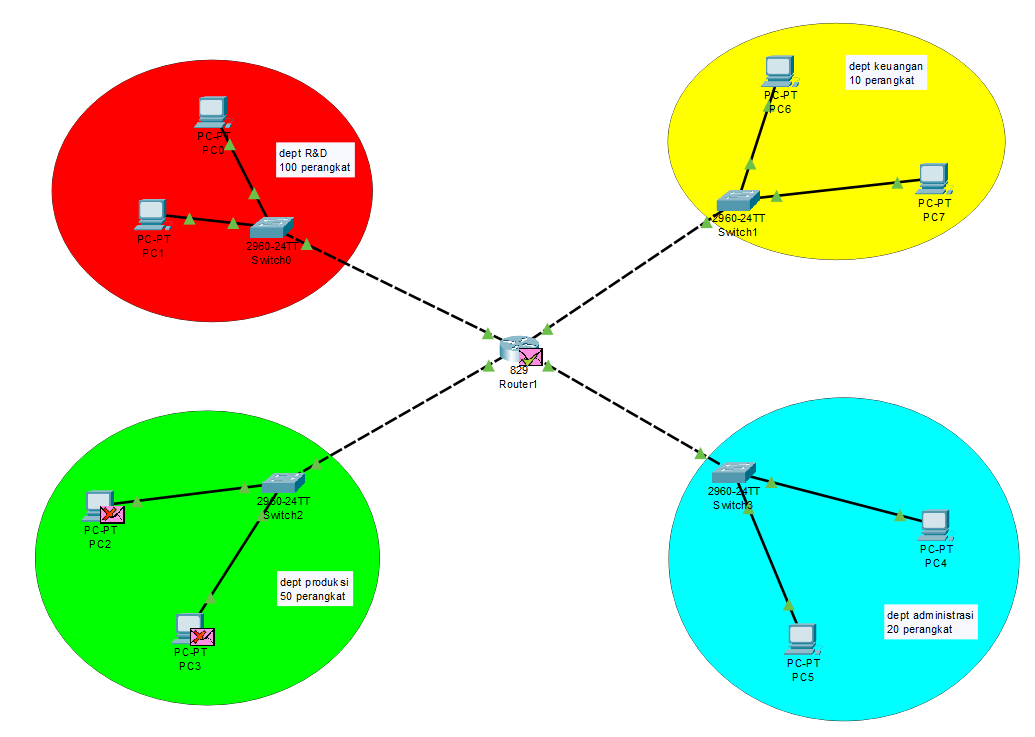
\includegraphics[scale=0.3]{P1/img/topology.png}
    \end{center}

    \item Jelaskan apa kesulitan yang anda alami pada Praktikum. \\
    Jawab: \\
    Kesulitan yang dialami pada praktikum ini antara lain pada saat crimping.
    Ada masalah saat memotong kabel LAN, di mana potongan terlalu pendek maka 
    kabel tidak dapat terhubung dengan baik. Selain itu, ada juga masalah pada 
    saat routing statis, di mana tidak dapat melakukan ping karena terblokir 
    oleh firewalll. Hal ini menyebabkan koneksi tidak dapat terhubung. Ada 
    masalah lain yang terjadi pada saat routing dinamis, di mana waktu 
    praktikum tidak cukup untuk menyelesaikan sampai tahap ping.
    
\end{enumerate}
\section{Kesimpulan}
Sesi praktik ini membantu memperkuat konsep crimping kabel serta perbedaan 
antara perutean statis dan dinamis. Pada aktivitas pertama, yang melibatkan 
crimping kabel LAN, hasil akhir menunjukkan bahwa dengan teknik yang tepat, 
koneksi yang stabil dan dapat diandalkan dapat dicapai. Hal ini sejalan 
dengan teori bahwa koneksi fisik yang kokoh sangat penting untuk memastikan 
kelancaran transmisi data dalam jaringan apa pun.

Percobaan perutean statis melibatkan konfigurasi alamat IP secara manual 
pada router dan laptop. Hasil ping yang berhasil menunjukkan bahwa data 
dapat berpindah antar perangkat tanpa masalah. Hal ini mendukung gagasan 
bahwa perutean statis menawarkan stabilitas jaringan, khususnya untuk 
pengaturan yang memanfaatkan IP tetap-seperti server atau sistem keamanan. 
Meskipun demikian, perutean statis juga memiliki kelemahan, terutama upaya 
ekstra yang diperlukan untuk mengkonfigurasi ulang perangkat setiap kali 
tata letak jaringan berubah.

Dalam pengaturan perutean dinamis, penggunaan DHCP memungkinkan alamat IP 
diberikan secara otomatis, dan protokol RIP memungkinkan router untuk 
berbagi informasi perutean. Hal ini membuat jaringan lebih mudah beradaptasi 
dan lebih mudah dikelola tanpa perlu memasukkan IP atau rute secara manual. 
Hasil ini mencerminkan apa yang telah dibahas dalam materi pembelajaran-
perutean dinamis secara umum lebih efisien dan terukur, terutama untuk 
jaringan yang lebih besar atau yang sering berubah.

Secara keseluruhan, percobaan ini dengan jelas menggambarkan perbedaan inti 
antara kedua pendekatan tersebut. Perutean statis memberi administrator 
kontrol penuh tetapi menuntut intervensi manual untuk setiap perubahan 
jaringan. Sebaliknya, perutean dinamis memungkinkan router untuk 
berkomunikasi dan menyesuaikan rute secara otomatis, menawarkan 
fleksibilitas yang lebih besar. Perutean statis bekerja paling baik untuk 
lingkungan yang sederhana dan stabil, sedangkan perutean dinamis ideal 
untuk jaringan yang perlu lebih responsif dan lebih mudah dipelihara.

\section{Lampiran}
\subsection{Dokumentasi saat praktikum}
    \begin{center}
        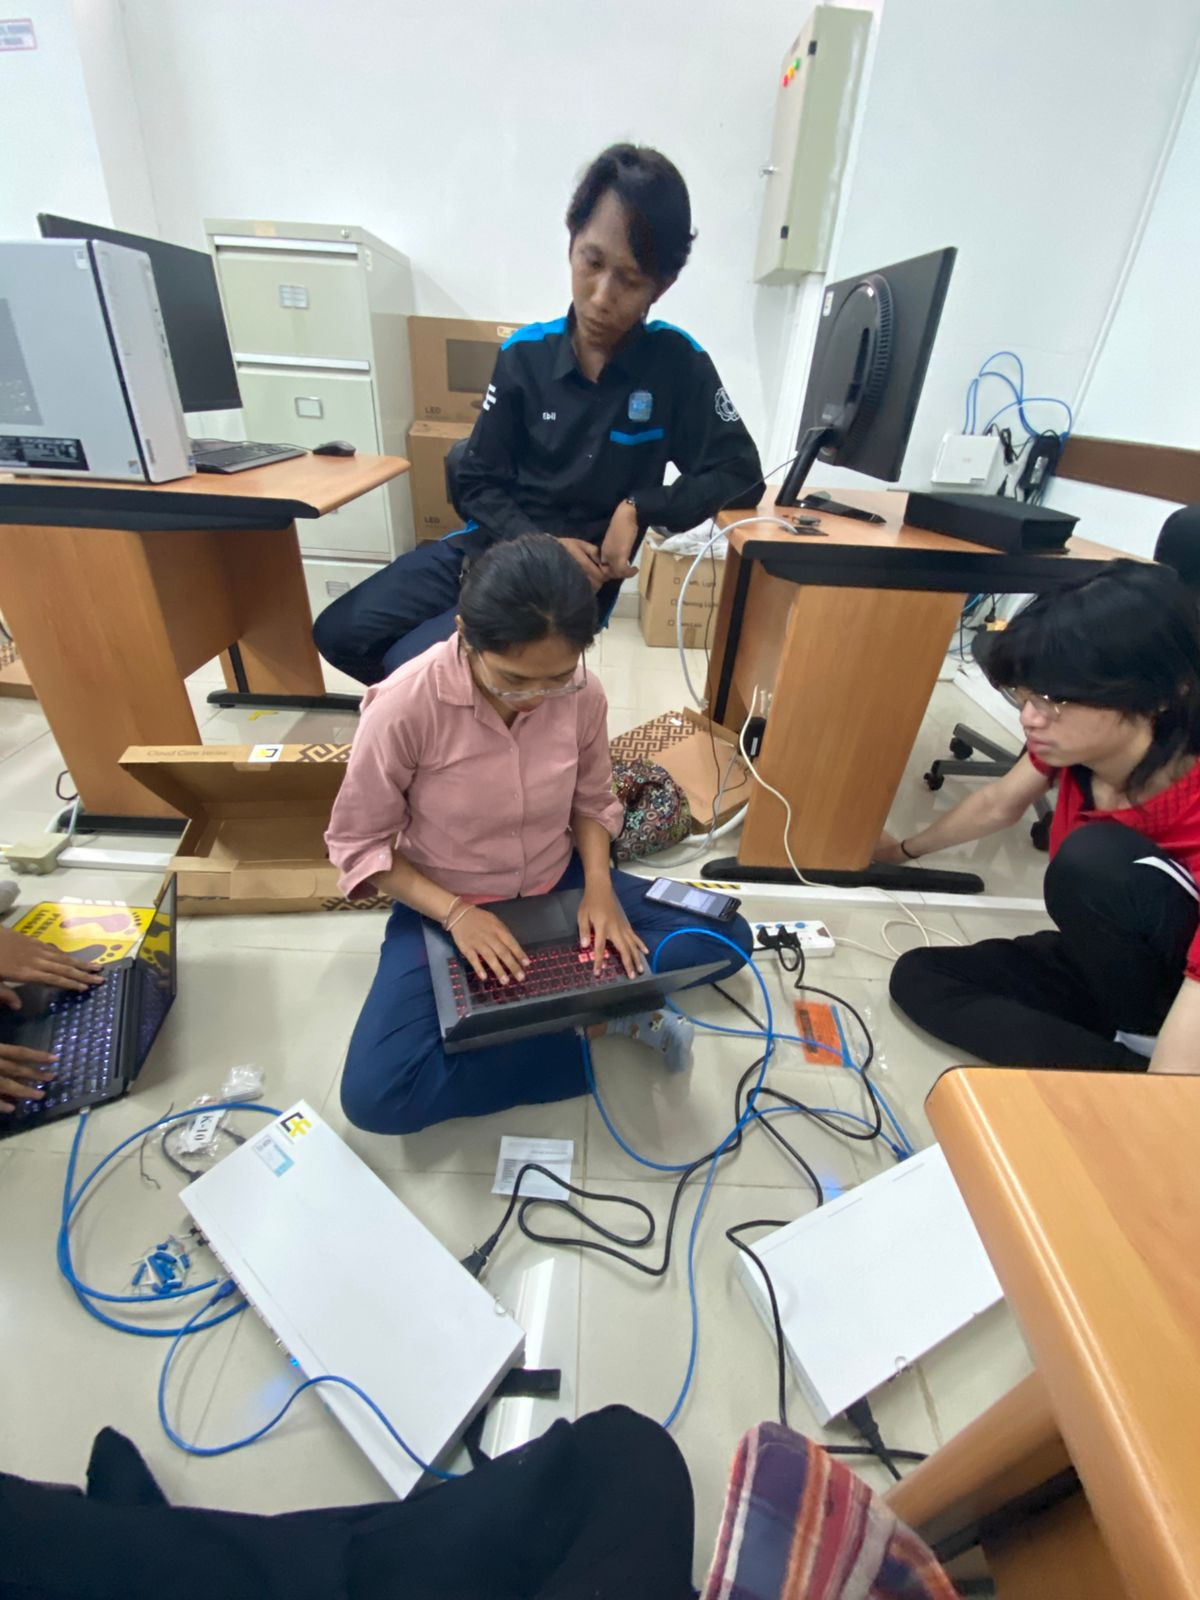
\includegraphics[scale=0.1]{P1/img/1-8.jpg}
    \end{center}
    \begin{center}
        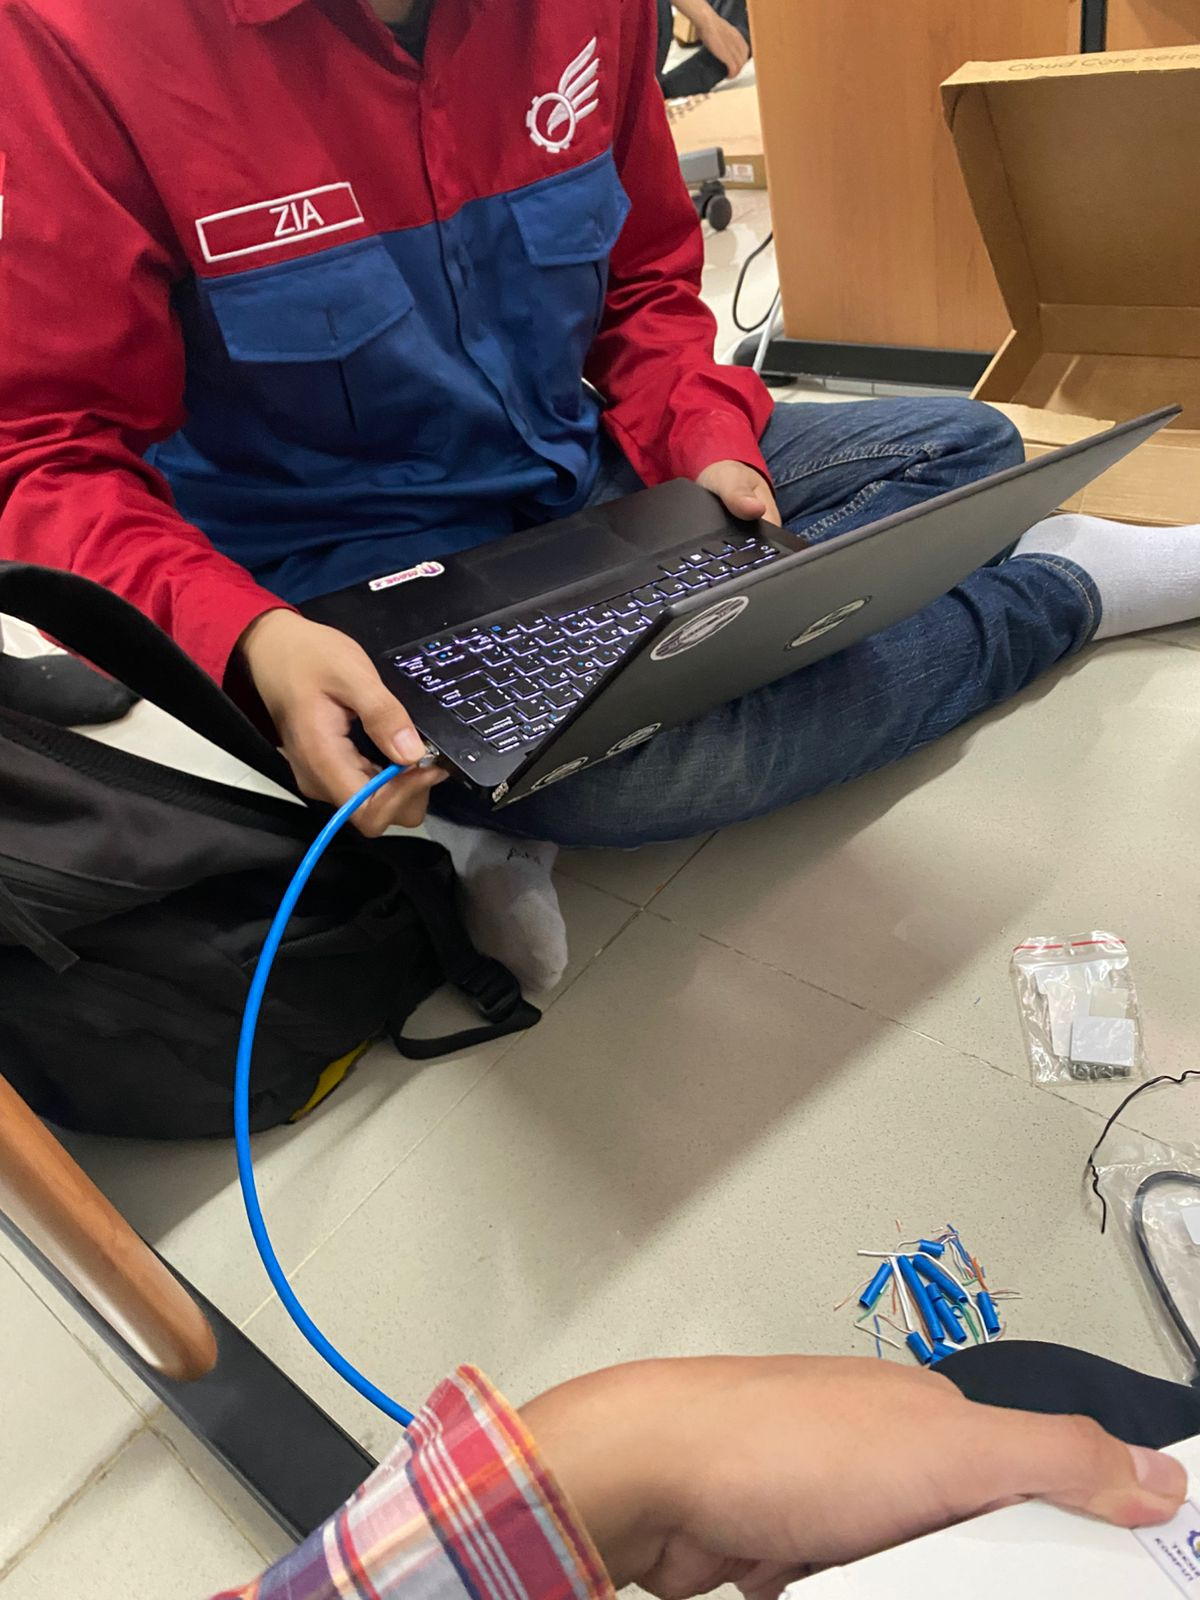
\includegraphics[scale=0.1]{P1/img/1-7.jpg}
    \end{center}
    \begin{center}
        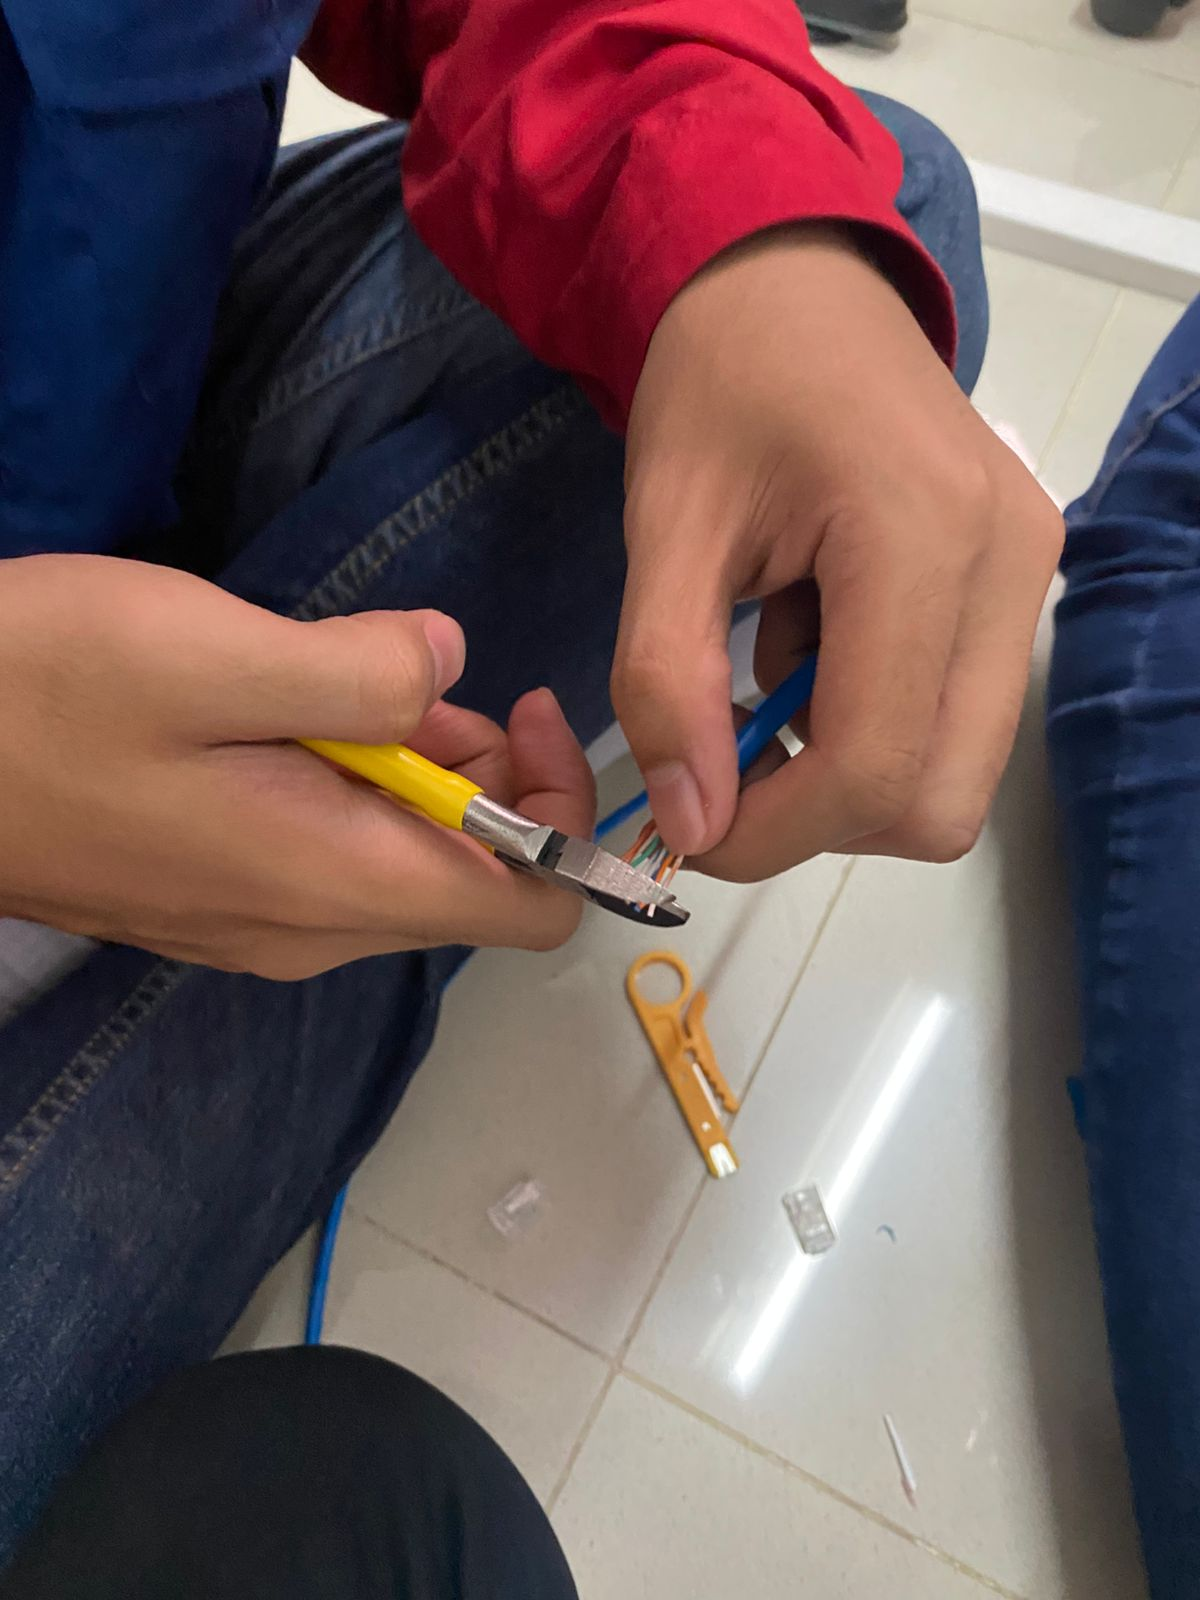
\includegraphics[scale=0.1]{P1/img/1-5.jpg}
    \end{center}